As our reliance on information technology continues to increase, the complexity and urgency of the problems our society will face in the future will increase much faster than are our abilities to understand and deal with them. It is expected that in the future, increasingly more complex applications will require very high computing performance and will process massive volume of data. Addressing these challenges requires radical changes in the way computing is delivered to support the computing requirements of these applications~\cite{sachs_ascr_2011}. New algorithms and programming models must be developed to enable significantly higher levels of parallelism. It is expected that the number of concurrent threads to sustain these required levels of parallelism will rise to a billion, a factor of 10,000 greater than what current platforms can support. This in turn will result in a massive increase in the number of computing cores, memory modules and storage components.

A direct implication of these emerging trends is the need to address the difficult challenge of minimizing energy consumption. Furthermore, the fault rates are expected to dramatically increase, possibly by several orders of magnitude~\cite{srinivasan_dsn_2004,torrellas2009architectures}. Figure~\ref{fig:sandia_system_mtbf} shows the system Mean Time Between Failures (MTBF) and the number of faults as a function of the number of nodes in the system~\cite{riesen_sandia_2010}. These faults, which can be transient, temporary, intermittent or permanent, stem from different causes and produce different effects. Concern about the increase of fault rates will not only be caused by the explosive growth in the number of computing and storage components, but will also grow out of the necessity to use advanced technology, operate at lower voltage levels, and deal with undesirable aging effects as they become significant~\cite{plank1995compressed}. Addressing this concern brings about unprecedented resilience challenges, which puts in question the ability of next generation HPC infrastructure to continue operation in the presence of faults without compromising the requirements of the supported applications. 


\begin{figure}[!t]
\begin{center}
	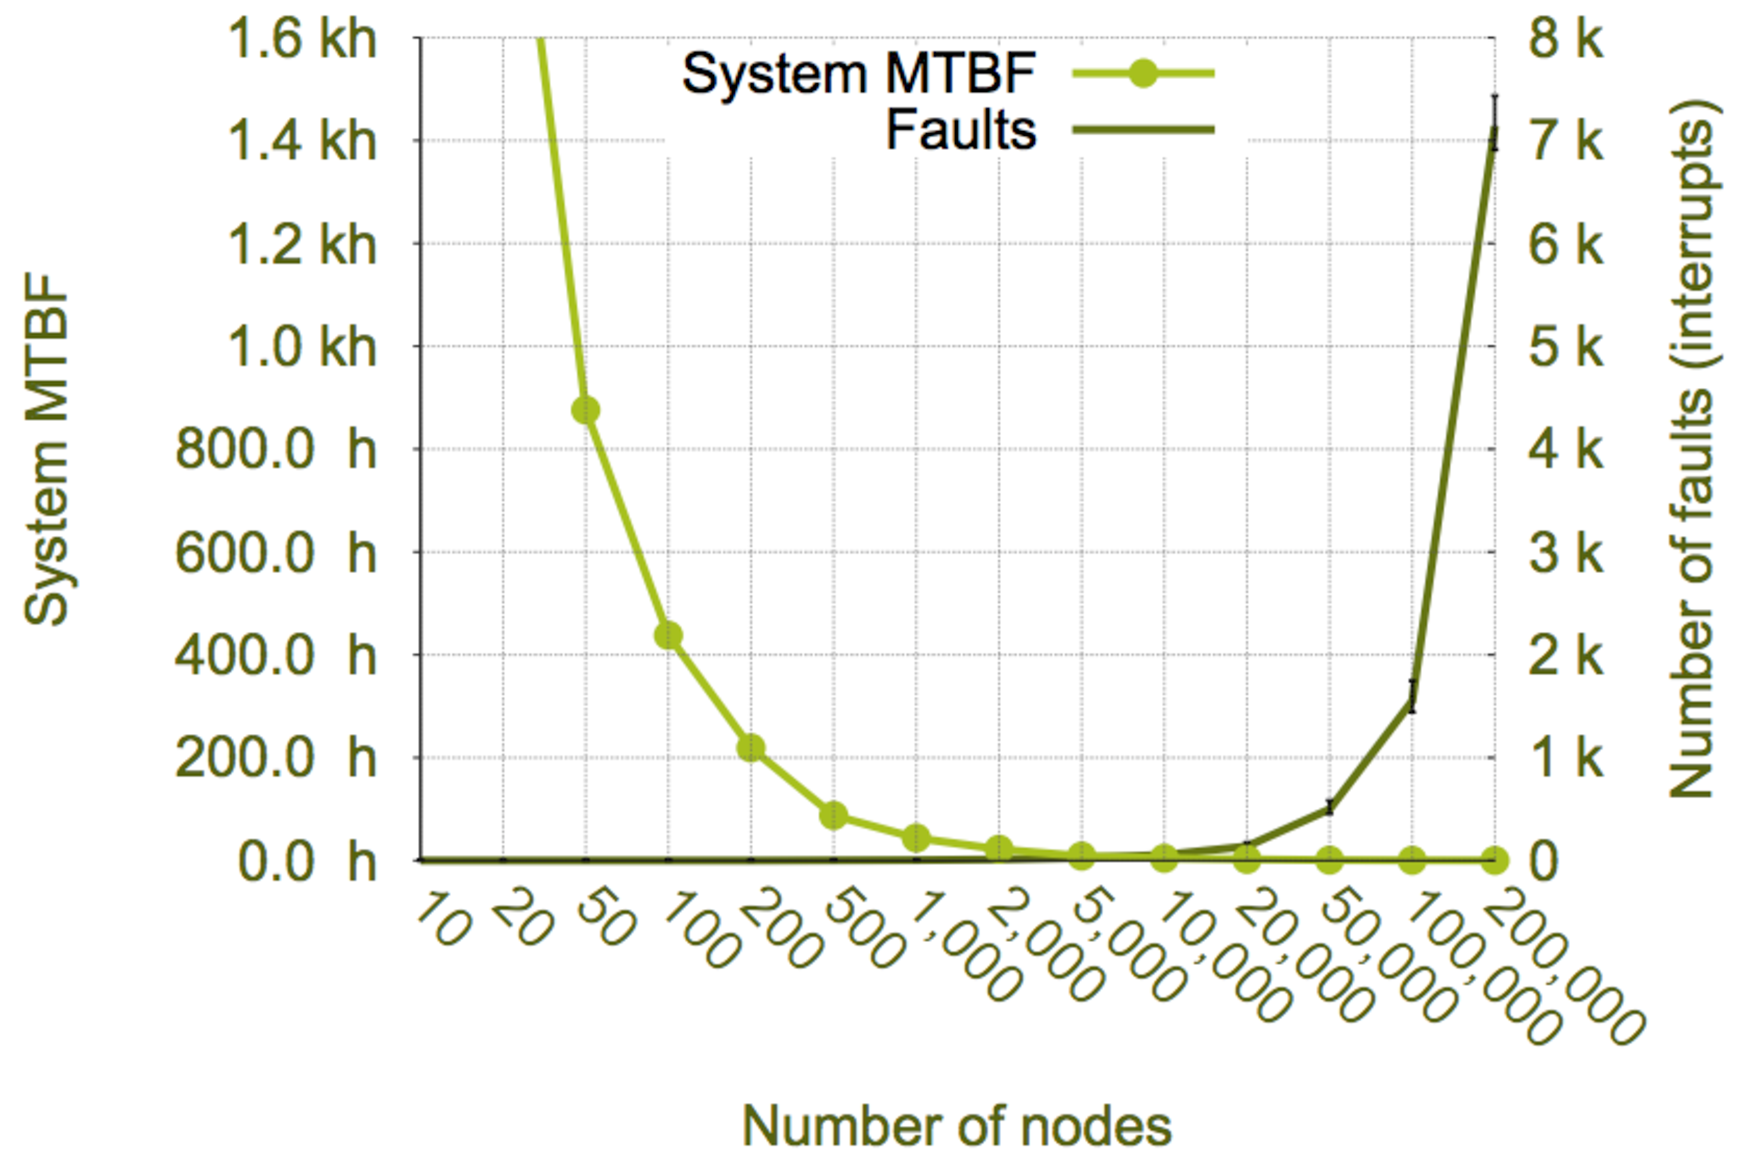
\includegraphics[width=\columnwidth]{figures/sandia_system_failure_rate_increase_nodes.pdf}
%\psfig{figure=diagrams/sandia_system_failure_rate_increase_nodes.eps,width=3.0in}
	\caption { Effect on system MTBF as number of nodes increase. }
	\label{fig:sandia_system_mtbf}
\end{center}
\end{figure}

The current response to faults consists of restarting the execution of
the application, including those components of its software
environment that have been affected by the occurring fault. To avoid
the full re-execution of the failing application, fault-tolerant
techniques typically checkpoint the execution periodically; upon the
occurrence of a hardware or software failure, recovery is achieved by
restarting the computation from a safe checkpoint. In some situations,
however, several components of the software environment associated
with the failed application may have to be restarted.

Given the anticipated increase in failure rate and the time required
to checkpoint large-scale compute- and data-intensive applications, it
is very likely that the time required to periodically checkpoint an
application and restart it upon failure may exceed the mean time
between failures.  Consequently, applications may achieve very little
computing progress, thereby reducing considerably the overall
performance of the system.  For example, a study carried out at Sandia
National Laboratories focused on evaluating the overhead incurred by
checkpointing. The results of the
study, depicted in Figure \ref{sandia_checkpoint_time}, clearly show
that beyond 50,000 nodes the application spends only a fraction of the
elapsed time performing useful computation.

\begin{figure}[!t]
\centering
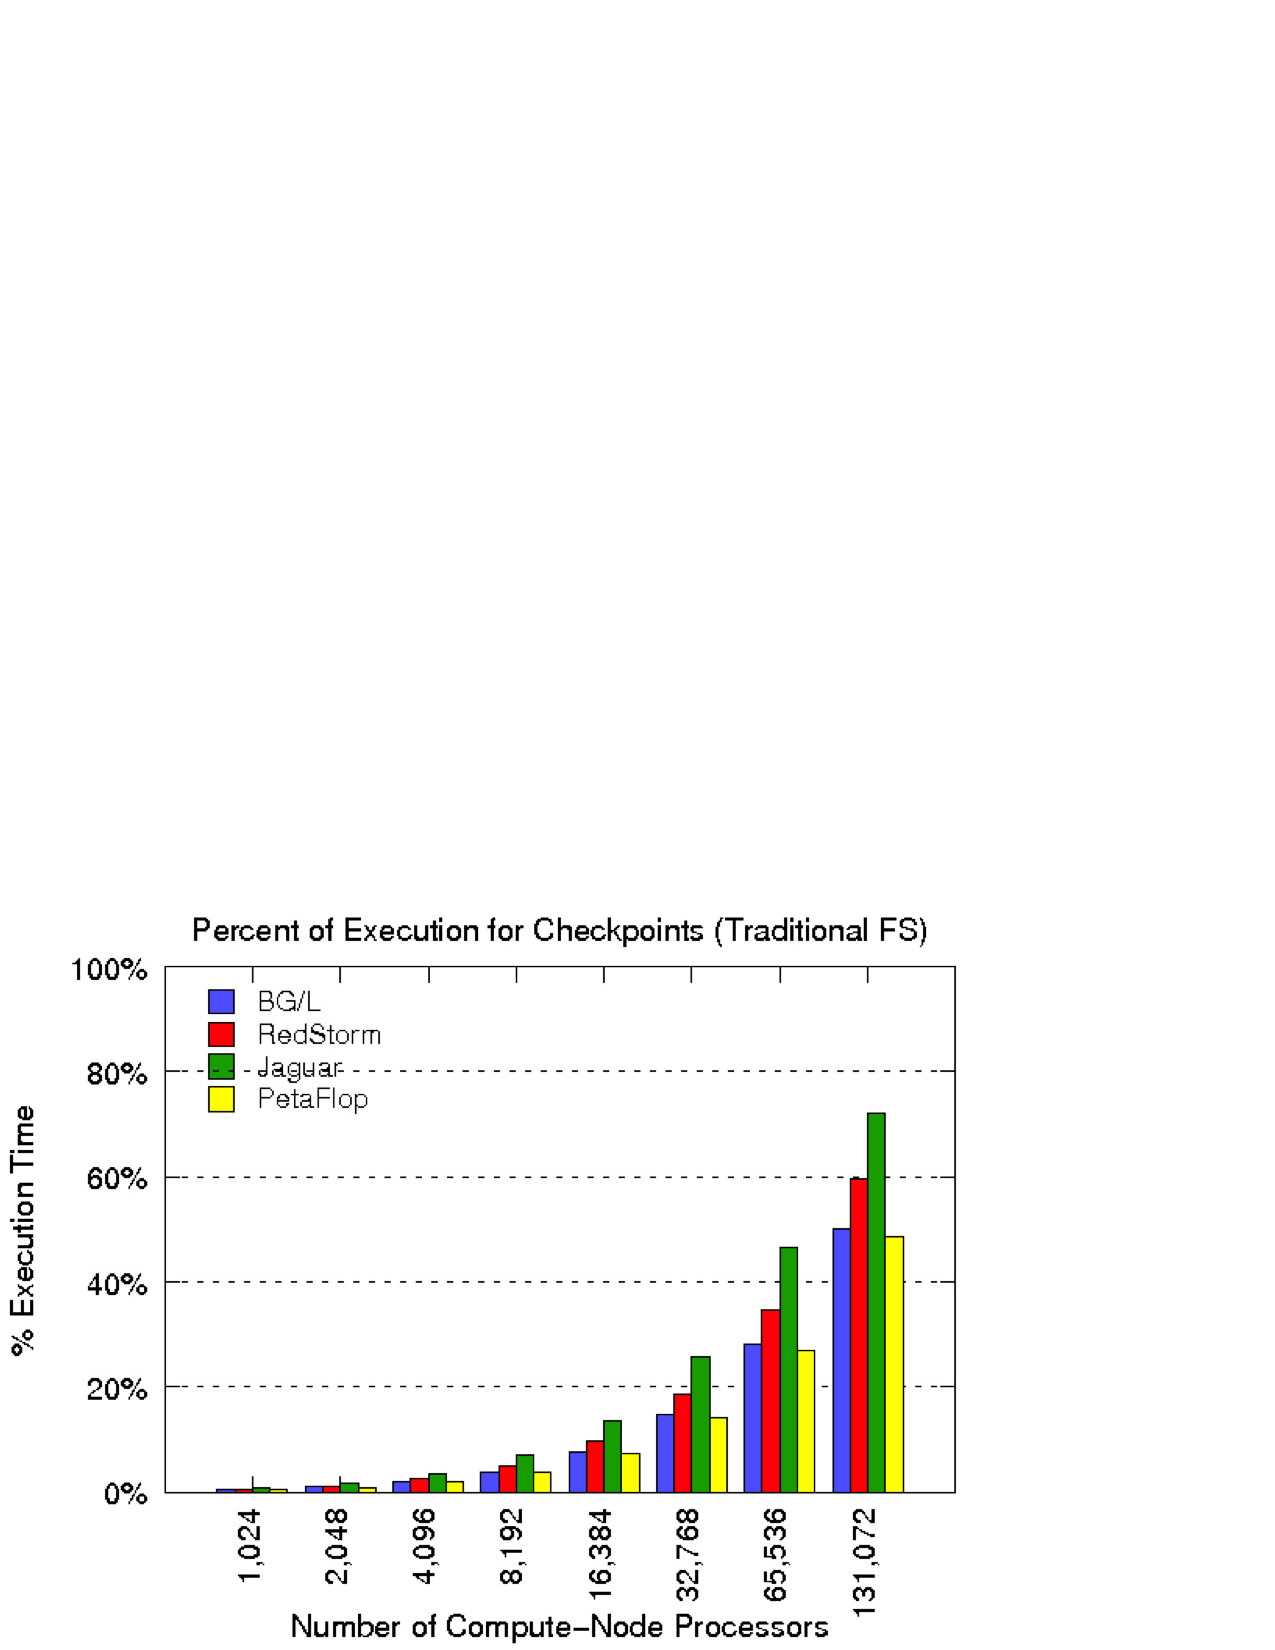
\includegraphics[width=\columnwidth]{figures/sandia_percent_of_time_for_checkpoints.pdf}
%\psfig{figure=diagrams/sandia_percent_of_time_for_checkpoints.eps,width=3.0in}
\caption { Percent of time to perform checkpoints. }
\label{sandia_checkpoint_time}
\end{figure}

%Current fault-tolerant frameworks are typically designed to handle single errors, whereas computation in large-scale, high-performance computing environments is likely to face multiple different types of errors, often concurrently. Even in the case of single errors, 
In addition, current fault-tolerant approaches apply the same technique, mainly checkpoint-restart over the entire duration of the execution, to handle all types of faults, including permanent node crashes, transient computing errors, and IO device failures. The nature of errors in large-scale, high-performance computing environments, however, are such that a general and expensive fault-tolerance technique, such as checkpoint-restart, may not be an adequate approach to handle the diverse types of faults in these environments. 

The main objective of this paper is to explore radically different
paradigms to enable scalable resiliency with minimum energy
consumption in future large-scale, high-performance computing environments. To this
end, we propose a new energy-aware ``lazy shadowing'' model, %as the
%basis for an efficient and scalable computational framework to achieve
%desired levels of fault tolerance, while minimizing energy
%consumption. The proposed model 
which goes beyond traditional checkpointing
and roll-back recovery techniques and uses a multi-level,
energy-aware replication approach to achieve scalable fault tolerance.

The basic idea of the lazy shadowing model is to associate with each
process a suite of ``shadow processes'', whose size depends on the
``criticality'' and performance requirements of the underlying
application. A shadow is an exact replica of the main process. In
order to overcome failure, the shadows are scheduled to execute
concurrently with the main process, but at different computing
nodes. Furthermore, in order to minimize energy, shadow processes
initially execute at decreasingly lower processor speeds. The
successful completion of the main process results in the immediate
termination of all shadow processes. If the main process fails, however,
the primary shadow process immediately takes over the role of the main
process and resumes computation, possibly at an increased speed, in
order to complete the task within the targeted response time. Moreover, one among the remaining shadow processes
becomes the primary shadow process.

In order to fully harness the potential of lazy shadowing to efficiently deal with failures, an optimization model is proposed to derive the execution rates of the main process and the prior- and post-failure execution rates of the shadow processes. The derived execution rates are such that the energy consumption is minimized, without violating the performance requirements of the underlying application. It is worth noting that the interplay between resilience and energy management manifests itself in different ways and must be analyzed carefully. Operating at lower voltage thresholds, for example, reduces power consumption but have adverse impact on the resilience of the system to handle high error rates in a timely and reliable fashion. Our approach will seek to avoid continuous change in voltage and frequency to prevent potential thermal and mechanical stresses on the electronic chips and board-level electrical connections. 

The remainder of the paper is organized as follows: Section
\ref{related_work} reviews work related to fault-tolerance in
large-scale high-performance computing systems. Section
\ref{model} presents the lazy shadowing framework and formulates an energy optimization problem
to achieve fault-tolerance, while minimizing energy consumption
without violating the expected performance requirements of the
supported application. In Section~\ref{application_to_hpc} two different approaches to
solving the energy optimization problem and their potential
implementation are explored. The methods differ in their approach to
energy minimization and their reaction to failures. In Section
\ref{analysis}, we develop a performance evaluation framework to
analyze and assess the performance of the three lazy shadowing
methods, including their sensitivity to critical workload and
performance parameters.  Throughout the study, the performance of the
two methods is compared to state machine replication, a recently proposed
alternative to check-pointing in large-scale HPC.  Section
\ref{conclusion} presents the conclusion of this work and discusses
future work.